\chapter{相關研究}
\label{cha:related_works}

我們所參考的文獻主要分為兩個類型,分別為程序化生成任務內容與程序化遊戲物件擺放。

\section{Mission/Space 框架}

Joris Dormans 認為一個完整的關卡需要包含任務與空間二者~\cite{dormans2010adventures}~\cite{dormans2011level}~\cite{dormans2012engineering};需要有一特定的空間佈局,及一系列需要於此空間中被執行的任務。關卡任務代表玩家需要按照任務流程,來依序挑戰才能夠完成該關卡;關卡的空間由其地理佈局所組成,或者由與地圖相似的節點網絡所構成。由於任務與空間之間的交錯混雜,導致關卡設計者最終採取簡單卻有效的策略,也就是讓任務與空間同構。雖然同構在設計上不是唯一的選擇,但對於某些遊戲是非常合適的,特別是一具有線性的關卡設計。而 Joris Dormans 亦提出了一種自動關卡設計的方法~\cite{dormans2010adventures}~\cite{dormans2012engineering},藉由產生一個任務,再利用這個任務去產生適合此任務的空間。舉例來說,關卡設計者透過生成任務的介面來建立任務圖 (mission graph),玩家必須執行這些任務才能夠完成關卡,接下來將任務轉換為空間,並將任務依序安排至該空間圖 (space graph) 中。設計者接著在地圖添加更細節的內容,直到地圖充滿任務的要素並作為遊戲的關卡。

任務圖注重於任務與玩家的相互關係,表現出玩家距離通關的進度狀況。主要由兩種要件:節點和有向連結線所構成,其中節點再細分為任務、起點與終點;有向連結線再依照兩節點之間的執行先後關係,細分為薄弱條件、強烈條件與抑制。其中,強烈條件或抑制的關係,會導致某些節點無法執行。空間圖直接呈現了關卡的空間結構,且大多數的節點能夠直接表示出玩家目前所在位置。空間圖中的任何節點能透過顏色、字母來表示不同類型。主要亦由兩種要件:節點和連結線所構成。節點細分為場所、鎖和遊戲元素所構成;有向連結線細分為通道、閥、窗、解鎖與上鎖等。

改寫系統 (rewrite system) 由具有左側與右側的規則 (rules) 所組成,能夠將規則中指定的一符號集能夠被另一符號集所取代。改寫規則當中所使用的符號,便是在遊戲中經常會出現一些具有代表性的物件、要素或任務目標等,在字母表 (alphabet) 中定義以抽象化描述遊戲中的週期性結構 (recurrent construction)。改寫系統能夠套用在構成任務的圖形語法 (graph grammars)及構成空間的形狀語法 (shape grammars),二者能夠獨立生成出結果,不過建議能夠將改寫系統套用在任務圖上,使其能夠產生出空間圖。本文提及之任務圖和空間圖是經過改良後的版本,定義其規則時會有些微上的不同,但更能夠體現出遊戲的關卡結構。

\section{Map Sketches 與 Segments 的演化}

Antonios Liapis 開發了策略型遊戲的抽象化地圖生成工具 - Sentient Sketchbook~\cite{liapis2013generating}。在 Sentient Sketchbook 中,遊戲關卡設計師能夠以低分辯率、高階抽象的方式來編輯地圖草圖 (map sketches),構成地圖的瓦磚類型有資源磚、基地磚、不可通行磚與可通行磚等。典型的戰略型遊戲中,每位玩家都必須從隨機選擇的基地開始採集資源以建構戰鬥單位,並利用這些戰鬥單位摧毀敵方基地以完成遊戲。

當設計師編輯地圖時,該工具能夠測試地圖的可玩性 (意旨能夠正常進行遊戲) 且量化顯示,如果沒有足夠的基地、資源或可連通的路徑,那麼工具提供的遊玩特徵指標將會提示該地圖為不可遊玩的狀態。而這些遊玩特徵指標分別為資源安全性:距離基地僅一格以內的資源磚數量;安全區域:計算基地與敵方基地間的磚總數;探索性:利用洪水填充演算法,計算從基地至敵方基地時,可通行的磚總數。透過用戶當前編輯的地圖草圖,該工具利用基因演算法進行前述等指標,評估適應性函數 (fitness functions) 以解決約束最佳化 (constrained optimization) 等問題,來產生出更多意想不到的地圖輸出結果。

後續的研究中,Antonios Liapis 將基因演算法調整為兩階段演化,第一階段演化為地圖草圖演化,第二階段為地圖片段 (map segments) 演化~\cite{liapis2017multi}。地圖片段的結構類似於地圖草稿,由 NxN 的瓦磚所構成,瓦磚的種類能夠像是空磚、牆、連接處、出口、怪物或寶箱等,其中連接處是為了讓地圖片段彼此能夠接合以填滿地圖。利用地圖草稿所轉化成的初始地圖片段可作為演化用的胚胎 (embryogeny),於此階段定義的牆、連接處會呈顯穩定狀態,不隨著演化過程而改變,其餘瓦磚有機會由空磚突變為怪物、寶箱或牆,反之亦然。並探討不同的目標函數與胚胎,如何影響的圖片段的最佳解與外觀。

\begin{figure}[t!]
  \begin{center}
    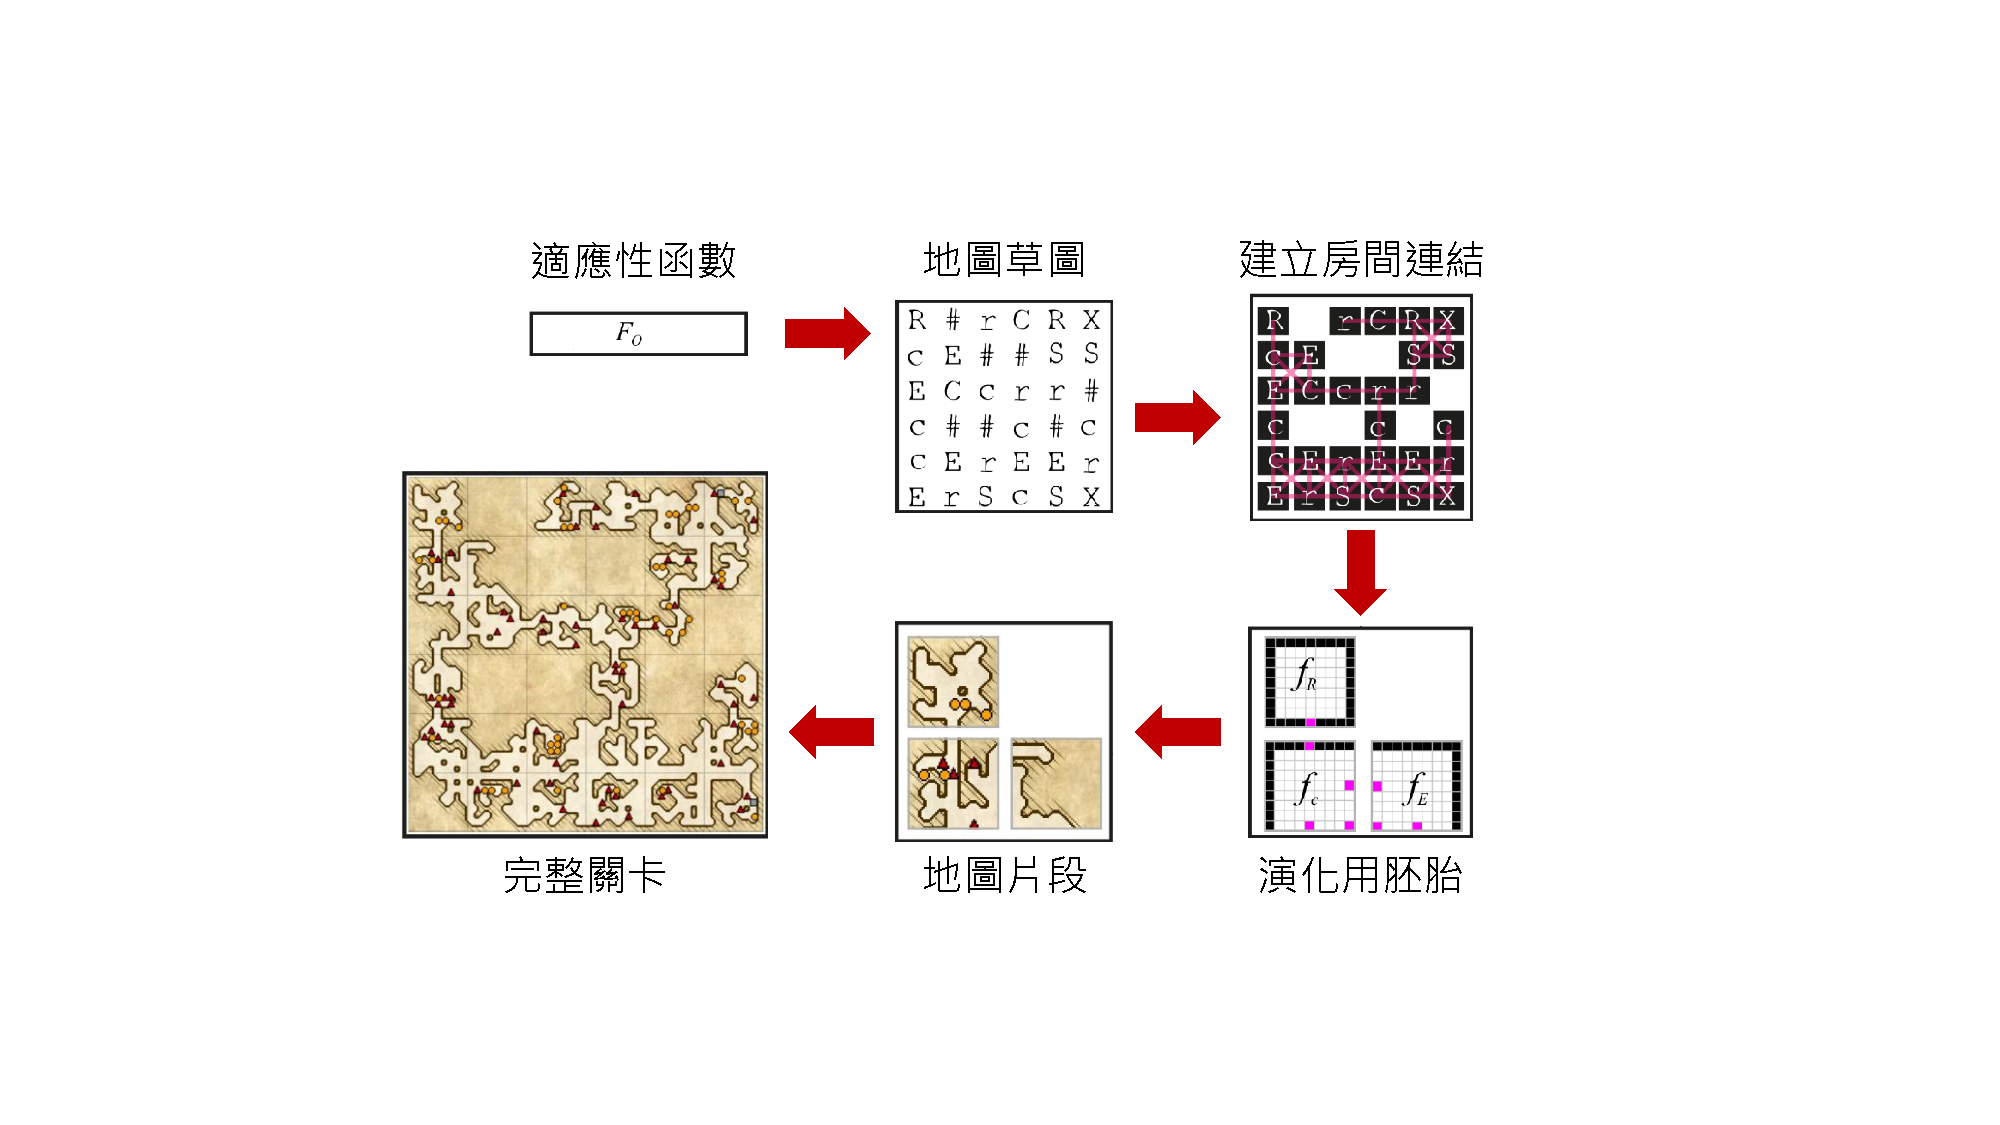
\includegraphics[width=1.0\textwidth]{figures/Multi-segment演化框架.pdf}
    \caption{Antonios Liaps 提出的兩階段式關卡演化。} 
    \label{fig:multi-segment-evolution}
  \end{center}
\end{figure}
